\section{Experiments}
\label{sec:experiments}

\paragraph{Scope and evidence discipline.}
All reported results come from the bundled run artifacts and are intentionally compute-aware: single seed (seed~0), a single main model (\texttt{EleutherAI/pythia-410m-deduped}), and a dev-model ablation block (\texttt{openai-community/gpt2}).
Whenever a baseline cell is missing in the artifacts (e.g., multiple COMPARE-2D baselines), we explicitly treat it as \emph{not run (compute scope)} and do not draw comparative conclusions from it.

\paragraph{Main outcomes across specs.}
Table~\ref{tab:main_runs} summarizes the four core specifications.
\Method closes all fully enumerable domains (COMPARE-2D, PARITY-4D, BALANCE-PAREN-14) with zero failures.
On the large-domain setting COMPARE-6D-STRAT, the certificate is \emph{coverage-bounded}: we evaluate a fixed stratified plan of $80{,}000$ prompts and report a certified pass rate of $0.862$ (Section~\ref{sec:certificates}).
Collateral metrics are reported for the gate-firing reference suites and vary materially by spec; in particular, PARITY-4D has low measured \KLS and moderate long-form drift, while COMPARE-2D and BALANCE-PAREN-14 exhibit higher measured drift under the same protocol.

\begin{table}[t]
\centering
\small
\setlength{\tabcolsep}{4pt}
\begin{tabular}{lrrrrrr}
\toprule
Spec & Total & Failures & Pass rate & Min margin & KL$_S$ & Drift$_L$ \\
\midrule
COMPARE-2D & 10000 & 0 & 1.000 & 1.00 & 9.694 & 1.000 \\
PARITY-4D & 10000 & 0 & 1.000 & 1.14 & 0.0017 & 0.125 \\
BALANCE-PAREN-14 & 32767 & 0 & 1.000 & 1.00 & 7.219 & 1.000 \\
COMPARE-6D-STRAT & 80000 & 11026 & 0.862 & -10.27 & 12.487 & 1.000 \\
\bottomrule
\end{tabular}
\caption{Main CertiPatch outcomes (reduced scope, seed 0). The first three specs are fully enumerable; COMPARE-6D-STRAT is coverage-bounded.}
\label{tab:main_runs}
\end{table}


\paragraph{Baseline comparisons where available (PARITY-4D).}
Table~\ref{tab:parity_baselines} compares \Method to completed baselines for PARITY-4D.
Several budget-matched PEFT baselines (LoRA, SoftPrompt, OneShot-FullDomain-MO) also close the spec in this run set (zero failures), but incur substantially larger measured collateral on the same gate-firing suites.
For example, \Method attains \KLS\ $=0.00168$ whereas LoRA reports \KLS\ $=0.01241$ and OneShot-FullDomain-MO reports \KLS\ $=0.11434$.
Long-form drift is similarly heterogeneous: LoRA and SoftPrompt drift on essentially all RefBool-L prompts, whereas \Method drifts on a strict subset (\DriftL\ $=0.125$).

\begin{table}[t]
\centering
\scriptsize
\setlength{\tabcolsep}{3pt}
\begin{tabular}{lrrrrrr}
\toprule
Method & Failures & $\KLS$ (mean) & 95\% CI & $\DriftL$ & FirstDiff & Params \\
\midrule
CertiPatch & 0/10000 & 0.00168 & [0.00165,0.00171] & 0.125 & 114.7 & 32768 \\
LoRA & 0/10000 & 0.01241 & [0.01219,0.01262] & 1.000 & 0.8 & 32768 \\
SoftPrompt & 0/10000 & 0.01881 & [0.01868,0.01896] & 0.999 & 3.0 & 32768 \\
OneShot-FullDomain-MO & 0/10000 & 0.11434 & [0.11304,0.11568] & 0.959 & 8.2 & 32768 \\
OneShot-FullDomain-ALM & 5000/10000 & 2.35966 & [2.35868,2.36064] & 1.000 & 0.0 & 32768 \\
SteeringVec-1L & 4868/10000 & 0.17692 & [0.17676,0.17708] & 0.022 & 125.2 & 1024 \\
Base & 5000/10000 & 0.00000 & [0.00000,0.00000] & 0.000 & 128.0 & 0 \\
\bottomrule
\end{tabular}
\caption{PARITY-4D comparison on the main model (single seed). All methods use the same Yes/No gate-scoped collateral suites. $\KLS$ is RefBool-S mean KL (base-to-patched) with bootstrap CI; $\DriftL$ is RefBool-L divergence rate and FirstDiff is the mean first-differing token index (128 means no difference within the generation budget).}
\label{tab:parity_baselines}
\end{table}

\paragraph{Baseline coverage gaps (COMPARE-2D).}
For COMPARE-2D, only the Base baseline cell is present in the artifacts; other baseline cells are missing because the required reference-suite artifact was not produced in this reduced bundle.
We therefore restrict COMPARE-2D discussion to (i) main-run outcomes and traces (Table~\ref{tab:main_runs}, Fig.~\ref{fig:cegis_trace}) and (ii) qualitative protocol properties (certificate semantics and compositionality).

\begin{figure}[t]
\centering
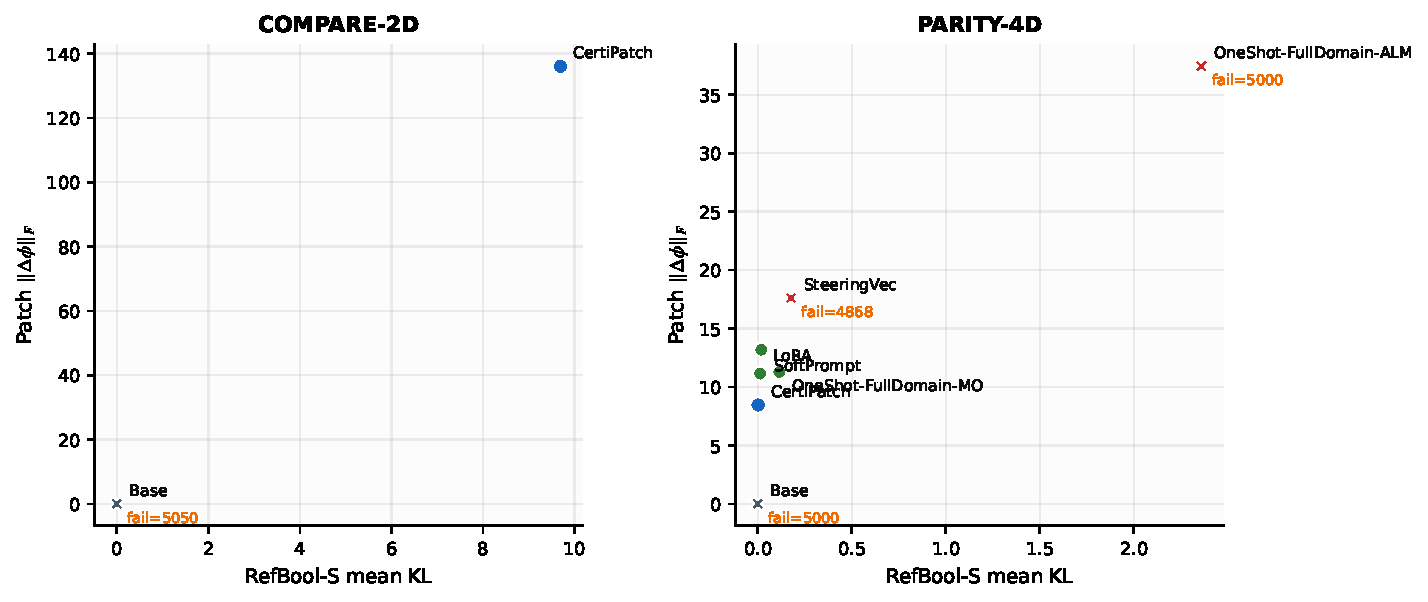
\includegraphics[width=0.98\linewidth]{figures/fig01_minimality_pareto.pdf}
\caption{Collateral vs patch complexity for COMPARE-2D and PARITY-4D (single seed). Points are annotated by method; infeasible cells show failure counts. Missing cells are treated as not run (compute scope) and do not appear.}
\label{fig:minimality_pareto}
\end{figure}

\begin{figure}[t]
\centering
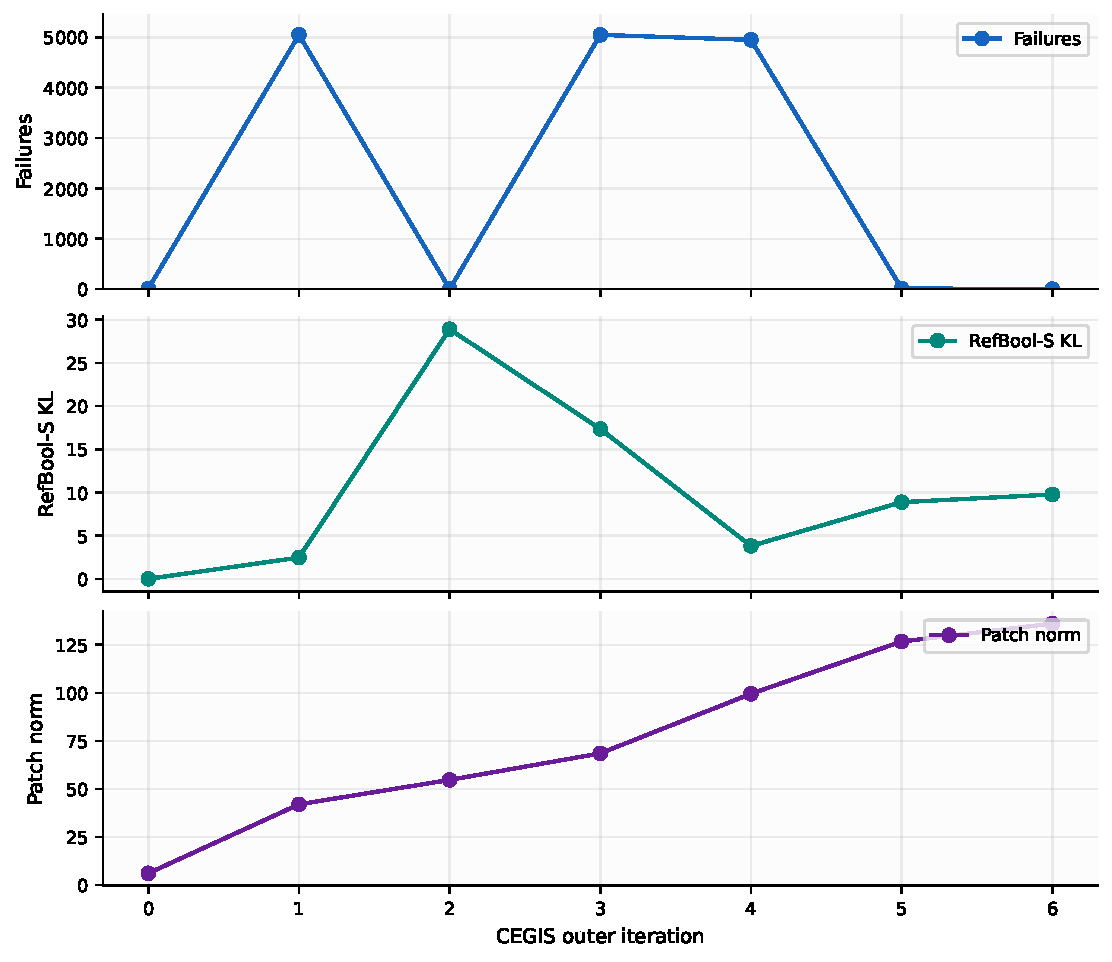
\includegraphics[width=0.94\linewidth]{figures/fig02_cegis_trace.pdf}
\caption{CEGIS dynamics on COMPARE-2D (single seed): spec failures, RefBool-S \KLS, and patch norm across outer iterations. This trace illustrates feasibility closure under counterexample-guided active-set growth; collateral behavior is reported, not assumed.}
\label{fig:cegis_trace}
\end{figure}

\paragraph{Coverage-bounded certification (COMPARE-6D-STRAT).}
Figure~\ref{fig:coverage_heatmap} reports failure rates across strata in the hashed coverage plan.
The certificate shows strong performance on boundary-focused strata (e.g., \texttt{S\_ext} and \texttt{S\_eq}) and weaker performance in several interior strata, emphasizing why this run is framed as \emph{coverage-bounded} rather than a full-domain claim.
A full strata table is provided in Appendix Table~\ref{tab:compare6d_strata}.

\begin{figure}[t]
\centering
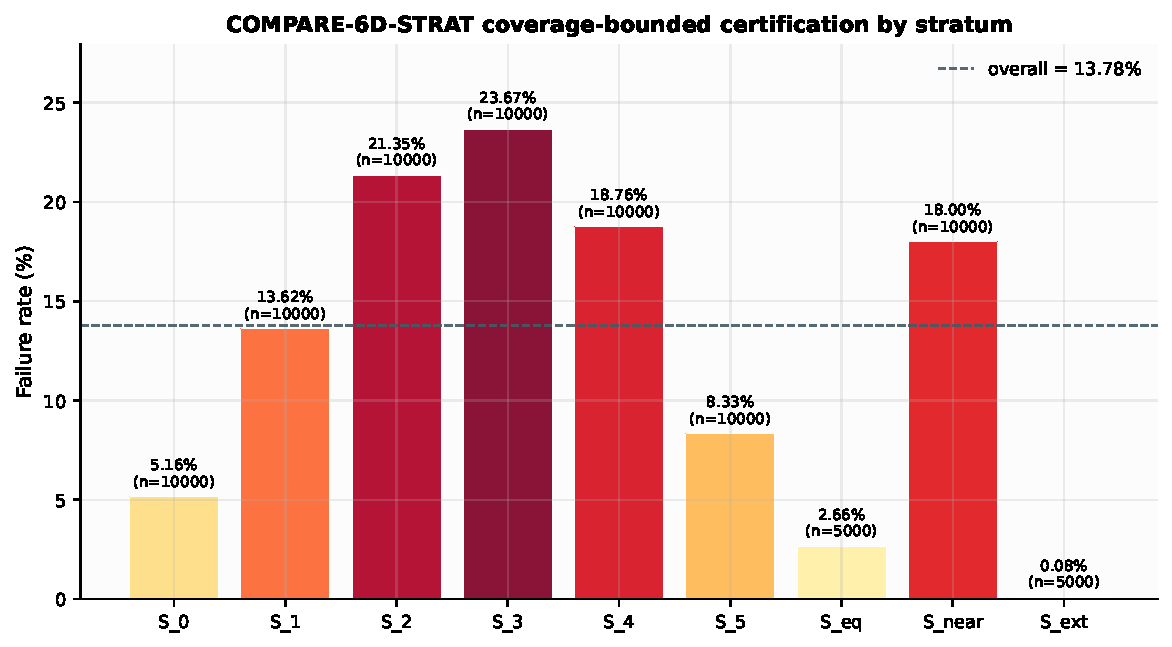
\includegraphics[width=0.98\linewidth]{figures/fig03_coverage_heatmap.pdf}
\caption{Coverage-bounded certification profile for COMPARE-6D-STRAT (single seed): certified failure rates per stratum (with stratum counts). The certificate claims only this coverage plan; out-of-coverage behavior is not certified.}
\label{fig:coverage_heatmap}
\end{figure}

\paragraph{Compositionality.}
We evaluate a six-condition compositionality suite using two specs: A (COMPARE-2D) and B (PARITY-4D).
Figure~\ref{fig:compositionality} shows strong order effects.
Naive additive composition (A$+$B) fails to transfer repair for spec~B (5{,}003 violations), while sequential repair (A$\to$B and B$\to$A) and joint repair recover zero failures on both specs.
These results indicate that patch interaction is non-commutative and must be measured rather than assumed.

\begin{figure}[t]
\centering
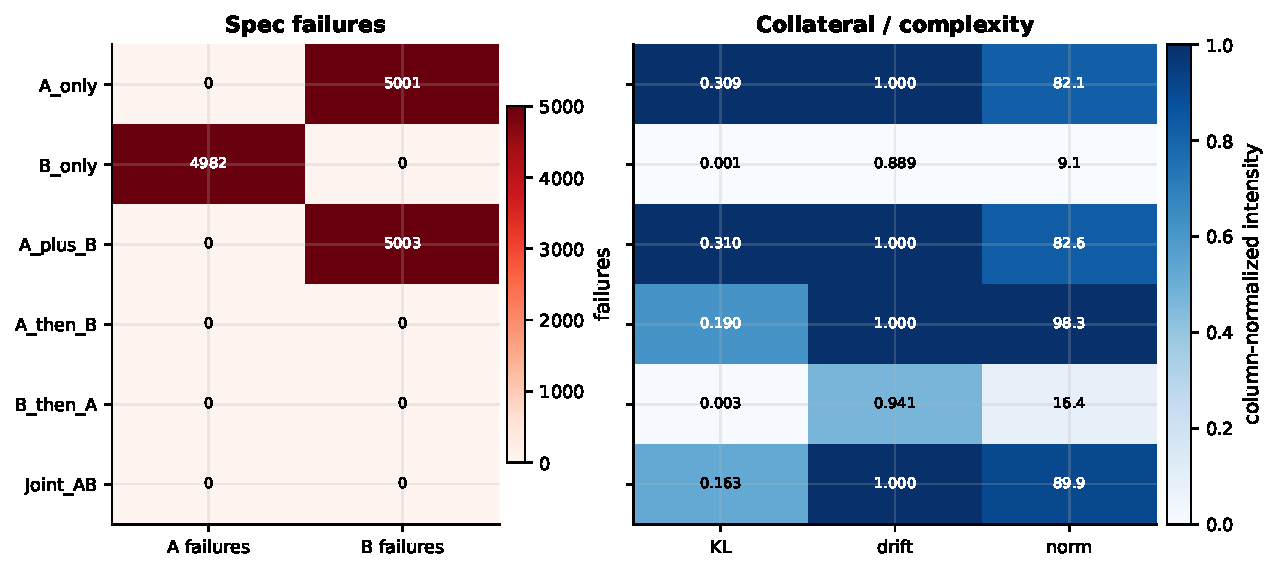
\includegraphics[width=0.94\linewidth]{figures/fig04_compositionality_matrix.pdf}
\caption{Compositionality matrix over six conditions (single seed): per-spec failures, collateral metrics, and patch norms. A$+$B denotes simultaneous application of the two independently learned patches; A$\to$B and B$\to$A denote sequential repair with feasibility constraints on both specs.}
\label{fig:compositionality}
\end{figure}

\paragraph{Verifier binding checks.}
Figure~\ref{fig:verifier_tamper} reports replay and tamper outcomes.
The verifier is fail-closed: replay passes only when the recorded hashes and scope definitions match regenerated artifacts, and controlled mismatches (patch perturbation, generator hash mismatch, coverage-plan hash mismatch, model revision mismatch) are rejected.

\begin{figure}[t]
\centering
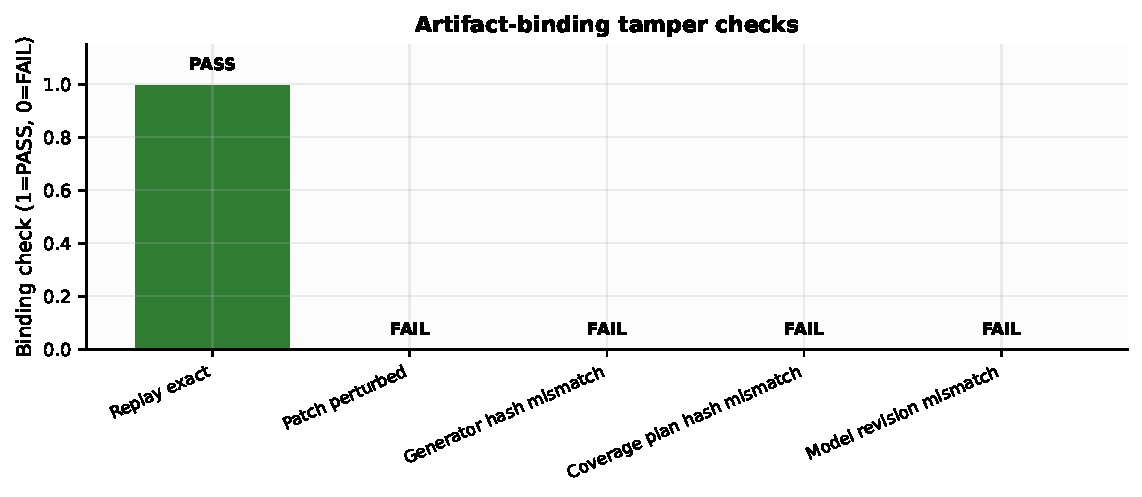
\includegraphics[width=0.98\linewidth]{figures/fig05_verifier_tamper.pdf}
\caption{Artifact-binding tamper checks. Replay-exact evaluation passes; each controlled tamper condition fails, consistent with fail-closed verifier semantics.}
\label{fig:verifier_tamper}
\end{figure}

\paragraph{Dev-model ablations (GPT-2).}
Table~\ref{tab:ablations} reports targeted ablations on the dev model for COMPARE-2D.
In this run set, constraining the patch to a single layer breaks feasibility closure, while several other ablations do not change the observed outcome.
We therefore treat these ablations as \emph{diagnostic} evidence for what is necessary in the small setting and avoid generalizing them beyond the reduced scope.

\begin{table}[t]
\centering
\small
\setlength{\tabcolsep}{5pt}
\begin{tabular}{lrrrrrr}
\toprule
Variant & Failures & Pass rate & KL$_S$ & Drift$_L$ & $\|\Delta\phi\|_F$ & Outer \\
\midrule
CertiPatch & 0 & 1.000 & 0.0011 & 0.527 & 7.64 & 7 \\
no\_minimality & 0 & 1.000 & 0.0011 & 0.527 & 7.64 & 7 \\
no\_cegis & 0 & 1.000 & 0.0011 & 0.527 & 7.64 & 1 \\
no\_collateral & 0 & 1.000 & 0.0011 & 0.527 & 7.64 & 7 \\
no\_gating & 0 & 1.000 & 0.0011 & 0.527 & 7.64 & 7 \\
rank\_1 & 0 & 1.000 & 0.0011 & 0.527 & 7.64 & 7 \\
single\_layer & 4849 & 0.515 & 0.0007 & 0.075 & 7.64 & 7 \\
random\_counterexamples & 0 & 1.000 & 0.0011 & 0.527 & 7.64 & 7 \\
\bottomrule
\end{tabular}
\caption{Dev-model ablations on GPT-2 (COMPARE-2D). In this run set, the single-layer constraint is the only variant that fails to close the spec.}
\label{tab:ablations}
\end{table}

\FloatBarrier
